\chapter{Experimentos} \label{chapter:chapter4}

En esta sección vamos a describir los experimentos realizados, el objetivo de cada uno de ellos y los resultados obtenidos.

\section{Experimento 1} \label{sec:exp1}

El objetivo de este experimento es buscar un enfoque para tratar de combinar las etiquetas de un conjunto $Y$ , tal que si $y_{j} \in Y, \cdots , y_{j + n} \in Y$ con  $n \leqslant |Y|$ se corresponden semánticamente en la imagen $x$ entonces elegir un representante $\hat{y} \in \{y_{j}, \cdots, y_{j+ n}\}$ tal que el nuevo conjunto de etiquetas es $\hat{Y} = \{ y_{0}, \cdots ,\hat{y}, \cdots , y_{|Y|}\}$. Para ponerlo en concreto vamos a dar un ejemplo de lo queremos alcanzar, para ello vamos a elegir una imagen con sus respectivas sentencias del conjunto de datos de \textit{COCO} captions como denota la Figura \ref{fig:exp1}, basándonos en la heurística detallada en la sección \ref{seccion:tags_gen} para obtener el conjunto de tags conseguimos que $Y = \{ $\textit{pastry}, \textit{frosting}, \textit{hand}, \textit{good}, \textit{man}, \textit{type}, \textit{close}, \textit{container}, \textit{kitchen}, \textit{baker}, \textit{chef}, \textit{person}, \textit{dessert}$\}$.


\begin{figure}
\begin{center}
    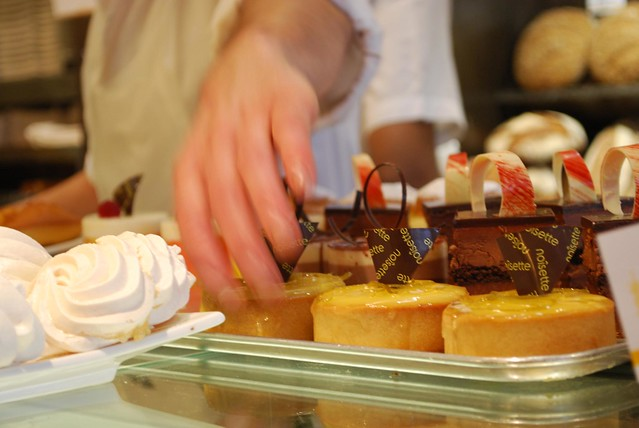
\includegraphics[width=\textwidth]{images/image208.jpg}
    \caption{Captions: \begin{itemize}
                             \item \textit{a chef is preparing and decorating many small pastries.}
                             \item \textit{a man preparing desserts in a kitchen covered in frosting.}
                             \item  \textit{a baker prepares various types of baked goods.}
                             \item  \textit{a close up of a person grabbing a pastry in a container}
                             \item \textit{close up of a hand touching various pastries.}
                      \end{itemize}}
    \label{fig:exp1}
\end{center}
\end{figure}

En base a este conjunto de palabras que representan a la imagen podemos decir que $y_{1} = \{\textit{baker}, \textit{chef}, \textit{person}, \textit{man}\}$ semánticamente representan lo mismo al igual que $y_{2}  = \{\textit{pastry}, \textit{dessert} \}$, por lo tanto un conjunto de datos óptimo sería $\hat{Y} = \{ \hat{y}_{1}, \hat{y}_{2}$, \textit{frosting}, \textit{hand}, \textit{good}, \textit{type},$ \textit{close}, \textit{container}, \textit{kitchen}\}$ donde $\hat{y}_{1}, \hat{y}_{2}$ son representantes de $y_{1} , y_{2}$ respectivamente.

Ahora ya sabemos el objetivo del experimento, nos resta dar la heurística utilizada para tratar dar con estas combinaciones de etiquetas, pero para ello primero veremos algunos conceptos claves en el enfoque para aproximar estas combinaciones, veremos mediante ejemplos lo que significa dentro de \textit{PLN} nociones como un árbol sintáctico de dependencias, \textit{POS} tagging y lematización. Primero veremos un tipo de árbol sintáctico de dependencia como lo es el \textit{DependecyParser} de \textit{Spacy} \footnote{\url{https://spacy.io/api/dependencyparser}} que está basado en las dependencias estándares de Stanford \cite{de-marneffe-etal-2014-universal} \footnote{\url{https://universaldependencies.org/u/dep/}}, en la Figura \ref{fig:Syntacti_parser} podemos ver el árbol de parseo sintáctico para la sentencia $c_{3}$ de la Figura \ref{fig:exp1} y en la Tabla \ref{tab:dep_s3_exp1} podemos ver las relaciones sintácticas expuestas en el ejemplo, básicamente cada token depende o está conectado con otro de la misma sentencia a través de una relación podemos definirlas como $R_{c} \subseteq \{(t_{1},t_{2}, rel )  |  t_{1},t_{2}  \in c  \land rel \in REL\}$ donde $REL$ es el conjunto de relaciones estándares. Otra noción importante y que se utilizará es \textit{POS} tagging \footnote{\url{https://spacy.io/usage/linguistic-features#pos-tagging}}, part of speech tagging por sus siglas en inglés, el cual consiste en predecir una categoría gramatical para cada palabra/token, por ejemplo en el ejemplo de la figura \ref{fig:Syntacti_parser} que vimos anteriormente en el ejemplo del parser, podemos notar que \textit{baker} tiene como categoría gramatical \textit{NOUN} lo cual es sustantivo en inglés. Por último otro concepto vastamente utilizado es la lematización  que consiste en quedarse con la raíz del token un ejemplo de esto puede ser \textit{prepare} para el token \textit{preparing}.

\begin{figure}
\begin{center}
    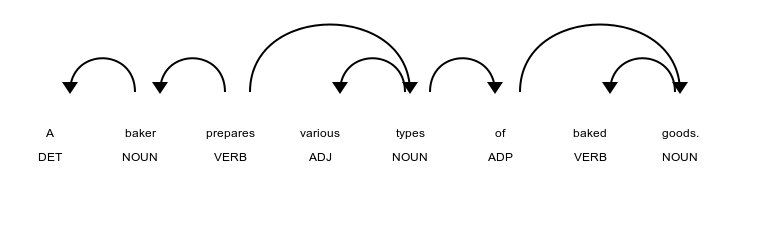
\includegraphics[width=\textwidth]{images/image218.png}
    \caption{Árbol de parseo sintáctico}
    \label{fig:Syntacti_parser}
\end{center}
\end{figure}

\begin{table}[ht]
    \centering
    \begin{tabular}{|c|c|c|}
        \hline
        \textbf{token} & \textbf{dependencia} & \textbf{ancestro}\\
        \hline \hline
        A & det & baker \\
        \hline
        baker & nsubj & prepares \\
        \hline
        prepares & ROOT & prepares \\
        \hline
        various &amod & types \\
        \hline
        types & dobj & prepares \\
        \hline
        of & prep & types \\
        \hline
        baked & amod & goods \\
        \hline
        goods & pobj & of \\
        \hline
    \end{tabular}
    \caption{Depenndencias de la sensencia $c_{3}$ de la Figura \ref{fig:exp1}}
    \label{tab:dep_s3_exp1}
\end{table}

Sea $C(x)$, $Y$ el conjunto de sentencias y el conjunto de tags ordenados correspondiente a la imagen x respectivamente que ya se describió en la sección \ref{seccion:tags_gen}, vamos a dar un algoritmo para generar $\hat{Y}$ el cual es el conjunto de tags ordenados utilizando la combinación de etiquetas.

Definamos \[KW_{x} = \{w | pos(w) \subseteq \{NOUN, VERB\}, w  \in c_{i}, c_{i} \in C(x) \}\] donde $pos(w)$ es una función que dado un token $w$ retorna su correspondiente $POS$ tagging, sea \[t_{i}= \{t_{i}^{1}, \cdots ,t_{i}^{m} \}\] tal que $lemma(t_{i}^{1}) = \cdots = lemma(t_{i}^{m})$ y $t_{i}^{j} \in KW_{x}$ donde $lemma(w)$ es una función que retorna la lematización del token dado, a partir de estos conjuntos vamos a generar otro conjunto de relaciones basados en la dependencia sintáctica, siguiendo con las definiciones sea 

\[RC = \{(rel, c_{k}) |  c_{k} \in child(t_{i}^{j}), t_{i}^{j} \in t_{i}, rel = reldep(t_{i}^{j}, c_{k}), rel \in REL \}\]

donde $reldep(w_{1}, w_{2})$ es una función donde dado dos token retorna su relación basado en el árbol sintáctico de dependencia y  $child(w)$ es una función donde retorna los hijos inmediatos en el árbol sintáctico para el token $w$. Ahora estamos en condiciones de dar un conjunto de tags el cual podemos combinar, sea

\[ M = \{y_{1}, \cdots , y_{n}\}\]

tal que $(rel, y_{i}) \in RC$, rel es la misma para todos los $y_{i}$ y por último $y_{i} \in Y$, pasándolo en limpio esto nos quiere decir que vamos a combinar aquellas etiquetas en las cuales tengan la misma relación en el árbol sintáctico y además están contenidas en el conjunto de tags inicial, solo nos resta la elección del representante $\hat{y} \in M $ y cómo será su score de relevancia $r$, $\hat{y}$ se selecciona de manera aleatoria entre los elementos de conjunto $M$, supongamos que $\hat{y}= y_{j}$ para $1 \leqslant j \leqslant n$ y su función $r$ está dada por 

\[r_{loc}(\hat{y}) = r_{loc}(y_{j})\]

\[ r_{freq}(\hat{y}) = \frac{ \sum_{i=1}^{n} \sum_{j=1}^{Q} count(y_{i}; c_{j})} { \sum_{k=1}^{Q} |t_{k}|} \]

por lo tanto:
\[r_{\alpha}(\hat{y}) = \alpha r_{freq}(\hat{y})+ (1 - \alpha) r_{loc}(\hat{y})\].

En la tabla \ref{tab:results_exp1} podemos ver los resultados de aplicar la heurística mencionada.

\begin{table}[ht]
    \centering
    \begin{tabular}{|c|c|c|c|c|c|c|}
        \hline
        \textbf{Métrica} &
        \textbf{Loss} &
        \textbf{$\alpha = 0$} &
        \textbf{$\alpha = 0.25$} &
        \textbf{$\alpha = 0.50$} &
        \textbf{$\alpha = 0.75$} &
        \textbf{$\alpha = 1$}\\
        \hline \hline
        p@1 & SJE1 & 0,4803 & 0,5838 & \textbf{0,6285} & 0,6187 & 0,5383 \\
        p@5 & SJE1 & \textbf{0,7043} & 0,7009 & 0,6977 & 0,6957 & 0,6773 \\
        p@1 & SJE2 & 0,4980 & 0,5931 & \textbf{0,6363} & 0,6287 & 0,5530 \\
        p@5 & SJE2 & \textbf{0,7307} & 0,7261 & 0,7206 & 0,7175 & 0,6963 \\
        p@1 & ListSJE & 0,4842 & 0,5706 & \textbf{0,6209} & 0,6182 & 0,5456 \\
        p@5 & ListSJE & 0,7539 & \textbf{0,7541} & 0,7540 & 0,7497 & 0,7179 \\
        \hline
    \end{tabular}
    \caption{Resultados}
    \label{tab:results_exp1}
\end{table}

A continuación veremos un par de ejemplos en los cuales estas combinaciones de etiquetas no funcionaron bien el cual nos servirá como puntapié para presentar el experimento número dos que veremos en la Sección \ref{sec:exp2}.


Aplicando la heurística para la Figura \ref{fig:bad_example_exp1} llegamos a combinar las siguientes etiquetas $\{\textit{egg}, \textit{bacon}\}$ como también $\{\textit{ham}, \textit{spinach}\}$lo cual no es correcto ya que no se corresponden semánticamente, en la Figura \ref{fig:Syntacti_parser_exp1_bad_example} podemos ver porque se llega a esta combinación para el segundo a través de su árbol de parseo sintáctico, esto nos dice que se combinan ya que $\{\textit{ham}, \textit{spinach}\} \in child(\textit{egg})$ y ambos están bajo la misma $rel = \textit{conj}$.

\begin{figure}
\begin{center}
    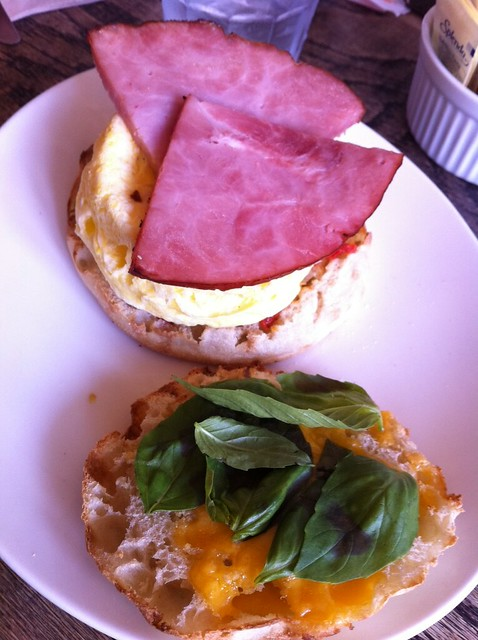
\includegraphics[width=\textwidth, height=120mm]{images/image203.jpg}
    \caption{Captions: \begin{itemize}
                             \item \textit{Plate with breakfast sandwich made with English muffin, egg and ham.}
                             \item \textit{a sandwich on a plate on a table}
                             \item  \textit{A white plate topped with a muffin filled with breakfast food.}
                             \item  \textit{A sandwich with egg and ham and spinach}
                             \item \textit{Two sandwiches on English muffins featuring greens and cheddar cheese on one sandwich and Canadian bacon and an egg on the other sandwich.}
                      \end{itemize}}
    \label{fig:bad_example_exp1}
\end{center}
\end{figure}

\begin{figure}
\begin{center}
    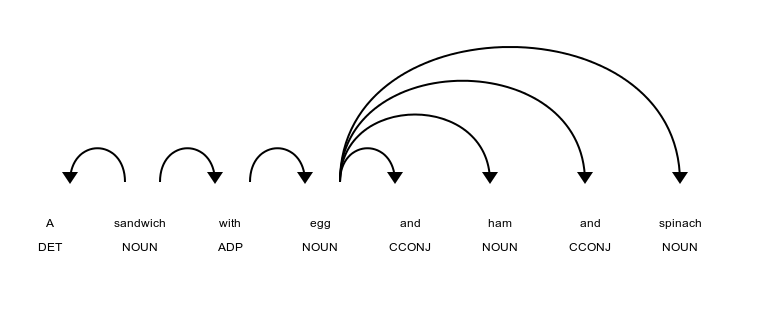
\includegraphics[width=\textwidth]{images/image198.png}
    \caption{Árbol de parseo sintáctico}
    \label{fig:Syntacti_parser_exp1_bad_example}
\end{center}
\end{figure}

\section{Experimento 2} \label{sec:exp2}

El objetivo del presente experimento es tratar de atacar las deficiencias obtenidas como conclusión al experimento detallado en la Sección \ref{sec:exp1}, para ello vamos a seguir combinando las etiquetas como lo mencionamos anteriormente pero con la salvedad de hacer un chequeo extra, el cual nos dice que se combinarán las etiquetas si y solamente si son hiperónimos de a pares.
Sea $Hyper(w_{1}, w_{2})$ un predicado el cual nos dice si el token $w_{2}$ es hiperónimo del token $w_{1}$ para realizar este chequeo hacemos uso de \textit{WordNet} \cite{worNet}, recordemos lo visto en la Sección \ref{sec:exp1} que $M$ es el conjunto de potenciales etiquetas a combinar, con esta referencia al experimento anterior vamos a combinarlas si se cumple la siguiente propiedad:
\[ \forall {w_{1},w_{2} \in M : Hyper(w_{1}, w_{2}) \lor Hyper(w_{2}, w_{1})} \]

Una vez realizado este chequeo extra se procede a elegir el representante $\hat{y} \in M$ y su score $r_{\alpha}(\hat{y})$ de la misma manera que lo visto en Seccion \ref{sec:exp1}.

En el Cuadro \ref{tab:results_exp2} podemos ver los resultados obtenidos.

\begin{table}[ht]
    \centering
    \begin{tabular}{|c|c|c|c|c|c|c|}
        \hline
        \textbf{Métrica} &
        \textbf{Loss} &
        \textbf{$\alpha = 0$} &
        \textbf{$\alpha = 0.25$} &
        \textbf{$\alpha = 0.50$} &
        \textbf{$\alpha = 0.75$} &
        \textbf{$\alpha = 1$}\\
        \hline \hline
        p@1 & SJE1 & 0,4703 & 0,5788 & 0,6332 & \textbf{0,6411} & 0,5646 \\
        p@5 & SJE1 & \textbf{0,6906} & 0,6856 & 0,6811 & 0,6808 & 0,6714 \\
        p@1 & SJE2 & 0,4885 & 0,5868 & 0,6420 & \textbf{0,6498} & 0,5784 \\
        p@5 & SJE2 & \textbf{0,7195} & 0,7145 & 0,7051 & 0,7019 & 0,6882 \\
        p@1 & ListSJE & 0,4758 & 0,5644 & 0,6244 & \textbf{0,6412} & 0,5719 \\
        p@5 & ListSJE & \textbf{0,7435} & 0,7434 & 0,7435 & 0,7401 & 0,7098\\
        \hline
    \end{tabular}
    \caption{Resultados}
    \label{tab:results_exp2}
\end{table}


\section{Experimento 3}

El objetivo de este experimento es reemplazar $\varphi = \textit{word2vec}$ por $ \varphi = \textit{BertEmb}_{BASE}$ y $\varphi = \textit{BertEmb}_{LARGE}$, a diferencia de lo visto en el Capítulo \ref{chapter:chapter3}, específicamente fijaremos $(\psi, \varphi) = (VGG19, BertEmb_{BASE})$ y $(\psi, \varphi) = (VGG19, BertEmb_{LARGE})$ como extractores de features visuales y textuales para el modelo descripto en la Ecuación \ref{eq:the_model}. Para la extracción de features textuales vamos a utilizar la última capa del encoder tanto de $\textit{BERT}_{BASE}$ como de $\textit{BERT}_{LARGE}$ utlizándolo como se detalló en la Sección \ref{sec:bert_emb}, para el resto de la sección nos vamos a abstraer de estos dos modelos y no vamos a discriminar entre $\textit{BERT}_{BASE}$ y $\textit{BERT}_{LARGE}$, luego en la exposición de resultados sí tendremos en cuenta cada modelo por separado. Ahora bien ¿Cómo a partir de \textit{BERT} llegamos a \textit{BertEmb}?, para ello vamos a detallarlo en el Algoritmo \ref{algo:bert_emb}, basicamente el diferencial de utilizar \textit{BERT} en vez de \textit{word2vec} es la generación de embeddings contextualizados, para un mismo token podemos tener varios embeddings que lo representen dependiendo del contexto de la sentencia en la cual el token ocurrió, en \textit{BertEmb} nos quedamos con el centroide de cada token del volcabulario en base a todas las ocurrencias del mismo.

\begin{algorithm}
\caption{\textit{BertEmb}}
\begin{algorithmic}[1]
\label{algo:bert_emb}
\STATE $BertEmb := dict()$
\STATE $temp := dict(list)$
\FOR{$set \in \{COCO_{train}, COCO_{val}\}$}
    \FOR{$(x, C(x)) \in set$}
        \FOR{$c_{i} \in C(x)$}
            \STATE $w_{1}^{v}, \cdots, w_{k}^{v} := \textit{BERT}(c_{i})$
            \STATE $temp[w_{j}] :+= w_{j}^{v}$ para $i=1, \cdots, k$
        \ENDFOR
    \ENDFOR
\ENDFOR
\STATE $BertEmb[w_{j}] := \textbf{mean}(temp[w_{j}])$ para $i=1, \cdots, |V|$ 
\end{algorithmic}
\end{algorithm}

Ahora que ya tenemos definido \textit{BertEmb} podemos dar los resultados de entrenar el modelo de la Ecuación \ref{eq:the_model} fijando  $(\psi, \varphi) = (VGG19, BertEmb_{BASE})$ y $(\psi, \varphi) = (VGG19, BertEmb_{LARGE})$, dichos resultados se exponen en los Cuadros \ref{tab:results_exp3_bert_1}, \ref{tab:results_exp3_bert_2} respectivamente.

\begin{table}[ht]
    \centering
    \begin{tabular}{|c|c|c|c|c|c|c|}
        \hline
        \textbf{Métrica} &
        \textbf{Loss} &
        \textbf{$\alpha = 0$} &
        \textbf{$\alpha = 0.25$} &
        \textbf{$\alpha = 0.50$} &
        \textbf{$\alpha = 0.75$} &
        \textbf{$\alpha = 1$}\\
        \hline \hline
        p@1 & SJE1 & 0.4581 & 0.5714 & 0.6306 & \textbf{0.6416} & 0.5683 \\
        p@5 & SJE1 & \textbf{0.685} & 0.6804 & 0.6778 & 0.6788 & 0.6673 \\
        p@1 & SJE2 & 0.4789 & 0.5832 & 0.6387 & \textbf{0.6499} & 0.5825 \\
        p@5 & SJE2 & \textbf{0.7149} & 0.7090 & 0.7018 & 0.6994 & 0.6849 \\
        p@1 & ListSJE & 0.4654 & 0.5604 & 0.6195 & \textbf{0.6422} & 0.5786 \\
        p@5 & ListSJE & 0.7400 & 0.7407 & \textbf{0.7408} & 0.7373 & 0.7095\\
        \hline
    \end{tabular}
    \caption{Resultados}
    \label{tab:results_exp3_bert_1}
\end{table}

\begin{table}[ht]
    \centering
    \begin{tabular}{|c|c|c|c|c|c|c|}
        \hline
        \textbf{Métrica} &
        \textbf{Loss} &
        \textbf{$\alpha = 0$} &
        \textbf{$\alpha = 0.25$} &
        \textbf{$\alpha = 0.50$} &
        \textbf{$\alpha = 0.75$} &
        \textbf{$\alpha = 1$}\\
        \hline \hline
        p@1 & SJE1 & 0.4598 & 0.5696 & 0.6281 & \textbf{0.6397} & 0.5684\\
        p@5 & SJE1 & \textbf{0.6850} & 0.6802 & 0.6773 & 0.6750 & 0.6637 \\
        p@1 & SJE2 & 0.4774 & 0.5809 & 0.6349 & \textbf{0.6480} & 0.5824 \\
        p@5 & SJE2 & \textbf{0.7130} & 0.7076 & 0.6978 & 0.6930 & 0.6818 \\
        p@1 & ListSJE & 0.4678 & 0.5608 & 0.6201 & \textbf{0.6402} & 0.5760 \\
        p@5 & ListSJE & \textbf{0.7385} & 0.7380 & 0.7384 & 0.7364 & 0.7073 \\
        \hline
    \end{tabular}
    \caption{Resultados}
    \label{tab:results_exp3_bert_2}
\end{table}


\section{Experimento 4} \label{sec:exp4}
La idea de este experimento es cambiar el modelo bilineal descripto en la Sección \ref{sec:model}, el cual siempre lo mantuvimos fijo, por uno que vamos a explayarnos a continuación y ver como impacta en los resultados.

El modelo que se utilizo queda expuesto en la Figura \ref{fig:exp4_custom_model} donde cada bloque de esta Arquitectura lo podemos ver en mayor detalle en el Cuadro \ref{tab:bloques_exp4_custom_model}, podemos ver que seguimos extrayendo features tanto visuales como de texto con \textit{VGG19} y \textit{word2vec} respectivamente. La noción de concatenar los embeddings transformados en el bloque $B3$ se toma desde la arquitectura propuesta en el paper \cite{DBLP:journals/corr/abs-1812-10546}.

\begin{figure}
\begin{center}
    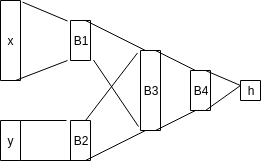
\includegraphics[width=\textwidth]{images/experiment4_model.png}
    \caption{Modelo del Experimento \ref{sec:exp4}}
    \label{fig:exp4_custom_model}
\end{center}
\end{figure}

\begin{table}[ht]
    \centering
    \begin{tabular}{|c|c|c|c|}
        \hline
        \textbf{Bloque} &
        \textbf{Composición} &
        \textbf{entrada} &
        \textbf{salida} \\
        \hline \hline
        x & VGG19 & - & 4096 \\
        y & word2vec & - & 300  \\
        B1 & $Dense + ReLU $ & 4096 & 300    \\
        B2 & $Dense + ReLU$ & 300 & 300  \\
        B3 & $ConCat + ReLU$ & (300, 300) & 600  \\
        B4 & $Dense + ReLU$ & 600 & 300 \\
        h  & $Dense + Linear$ & 300 & 1 \\
        \hline
    \end{tabular}
    \caption{Bloques}
    \label{tab:bloques_exp4_custom_model}
\end{table}

Los resultados obtenidos se muestran en el Cuadro \ref{tab:results_exp4_custom_model}, como podemos ver no hay muchas diferencias que utlizar el modelo bilineal.

\begin{table}[ht]
    \centering
    \begin{tabular}{|c|c|c|c|c|c|c|}
        \hline
        \textbf{Métrica} &
        \textbf{Loss} &
        \textbf{$\alpha = 0$} &
        \textbf{$\alpha = 0.25$} &
        \textbf{$\alpha = 0.50$} &
        \textbf{$\alpha = 0.75$} &
        \textbf{$\alpha = 1$}\\
        \hline \hline
        p@1 & SJE1 & 0.4336 & 0.5501 & 0.607 & \textbf{0.6189} & 0.5392\\
        p@5 & SJE1 & \textbf{0.6749} & 0.6695 & 0.6682 & 0.6702 & 0.6677 \\
        p@1 & SJE2 & 0.4715 & 0.5728 & 0.6262 & \textbf{0.6394} & 0.575 \\
        p@5 & SJE2 & \textbf{0.7209} & 0.7169 & 0.7057 & 0.7029 & 0.6915 \\
        p@1 & ListSJE & 0.4632 & 0.56 & 0.6188 & \textbf{0.6378} & 0.5742 \\
        p@5 & ListSJE & 0.7474 & \textbf{0.7482} & 0.7477 & 0.7436 & 0.7141 \\
        \hline
    \end{tabular}
    \caption{Resultados}
    \label{tab:results_exp4_custom_model}
\end{table}


\section{Experimento 5} \label{sec:exp5}

El presente experimento se enfocará en encontrar una representación conjunta, tanto para la imágen como para el tag, a través de un \textit{Autoencoder} para luego a partir de esto poder entrenar un modelo lineal, regresor, que nos estima el score que antes obteníamos con $s_{( \psi, \varphi)}(x, y ;W)$.
En la Figura \ref{fig:exp5_autoencoder} podemos ver la arquitectura del \textit{Autoencoder}, llamemos a este modelo \textbf{AutoEnc}, para el diseño de la misma nos basamos en la arquitectura del paper \cite{2019arXiv190405985W}, la idea es reconstruir la salida tanto la imágen como el tag que esta toma como entrada. En el Cuadro \ref{tab:bloques_exp4_custom_model} podemos ver la definición de cada bloque de la Figura \ref{fig:exp5_autoencoder}. Para entrenar este modelo se utlizó el mismo conjunto de entrenamiento y validación con la generación de tags descripta en el Capítulo \ref{chapter:chapter3}.

Ahora bien, una pregunta interesante es ¿cómo está definida la función de pérdida para este modelo?, se la definió como la suma de los \textit{mse} de cada uno:
\[L_{AutoEnc}(x, y) = mse(x, x') + mse(y, y')\]
donde $x'$, $y'$ son la salida de $AutoEnc$ y \textit{mse} es el error cuadrático medio.

Una vez que tenemos \textit{AutoEnc} entrenado procedemos a extraer esta representación conjunta para una imágen y un tag del bloque $B4$ y a partir de esta representación entrenamos un modelo lineal para estimar el score de relevancia expuesto anteriormente. En el Cuadro \ref{tab:results_exp5_autoencoder} podemos ver los resultados obtenidos en este experimento.


\begin{figure}
\begin{center}
    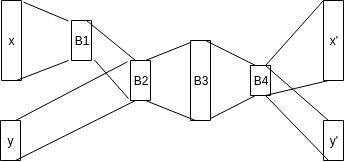
\includegraphics[width=\textwidth]{images/autoencoder_arch.png}
    \caption{Modelo del Experimento \ref{sec:exp5}}
    \label{fig:exp5_autoencoder}
\end{center}
\end{figure}


\begin{table}[ht]
    \centering
    \begin{tabular}{|c|c|c|c|}
        \hline
        \textbf{Bloque} &
        \textbf{Composición} &
        \textbf{entrada} &
        \textbf{salida} \\
        \hline \hline
        x & VGG19 & - & 4096 \\
        y & word2vec & - & 300  \\
        B1 & $Dense + ReLU $ & 4096 & 300    \\
        B2 & $Dense + ReLU$ & (300, 300) & (300, 300)  \\
        B3 & $ConCat$ & (300, 300) & 600  \\
        B4 & $Dense + ReLU$ & 600 & 200  \\
        $x'$ & $Dense + Linear$ & 200 & 4096 \\
        $y'$ & $Dense + Linear$ & 200 & 300 \\
        \hline
    \end{tabular}
    \caption{Bloques}
    \label{tab:bloques_exp4_custom_model}
\end{table}


\begin{table}[ht]
    \centering
    \begin{tabular}{|c|c|c|}
        \hline
        \textbf{Métrica} &
        \textbf{Loss} &
        \textbf{$\alpha = 0.50$}\\
        \hline \hline
        p@1 & SJE1 & \textbf{0.2329} \\
        p@5 & SJE1 & \textbf{0.5643} \\
        \hline
    \end{tabular}
    \caption{Resultados}
    \label{tab:results_exp5_autoencoder}
\end{table}